%!TEX root = ../thesis.tex
%Adding the above line, with the name of your base .tex file (in this case "thesis.tex") will allow you to compile the whole thesis even when working inside one of the chapter tex files


\chapter{Observation and Instrumentation} 
\label{chap:3}

\section{Thompson Scattering Theory}\label{sec:1}

\subsection{Thomson Scattering in the Corona}\label{sec:10}

The first evidence for the existence of the corona was through observations during solar eclipses. The occultation of the solar disk by the moon revealed a visible outer atmosphere structured into streamers and plumes and extending far from the solar surface (Fig.~\ref{fig:eclipse}). This is known as the white-light corona and is due to Thomson scattering of photospheric light by free electrons in the corona.
\begin{figure}[t!]
\begin{center}
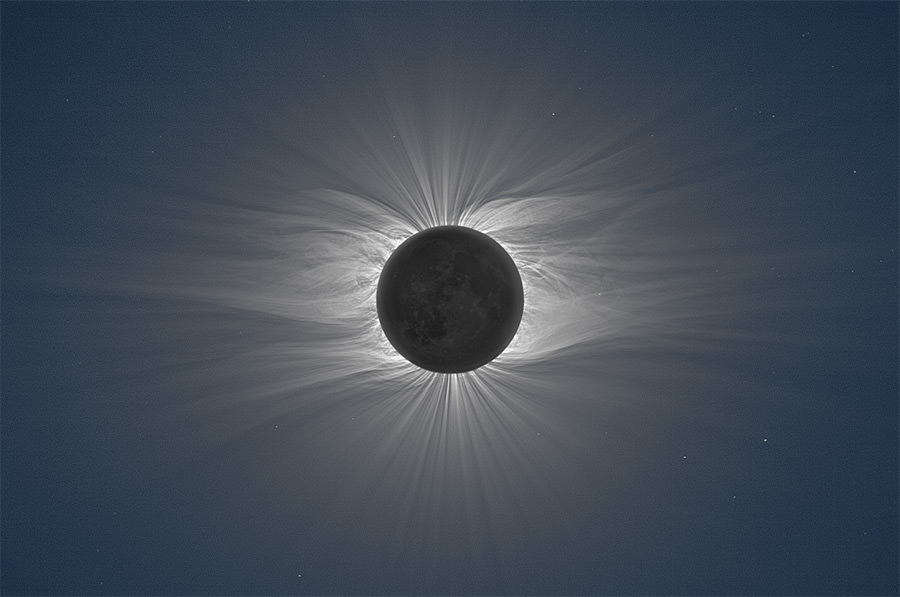
\includegraphics[scale=0.45]{images/solar_eclipse}
\caption[White-light corona during an eclipse]{The white-light corona during a solar eclipse. Occultation of the bright solar disk by the moon reveals the faint outer atmosphere of the Sun, known as the corona. It is highly structured, showing features like streamers and plumes. {\it Eclipse photograph courtesy of Miloslav Druckm\"{u}ller \href{http://www.zam.fme.vutbr.cz/~druck/Index.htm}{http://www.zam.fme.vutbr.cz}}}
\end{center}
\label{fig:eclipse}
\end{figure}

The tangential component ($I_T$), radial component ($I_R$), and polarization ($I_P$) of the scattered intensity are given by the expressions
\begin{equation}
I_T=I_0\frac{\pi \sigma_e}{2z^2}[(1-u)C +uD]
\end{equation}

\begin{equation}
I_P=I_0\frac{\pi \sigma_e}{2z^2}\mathrm{sin}^2\chi[(1-u)A +uB]
\end{equation}
with $I_R = I_T-I_P$. $A$, $B$, $C$, and $D$ are the van de Hulst coefficients and are a trigonometric function only of the solid angle subtended by the Sun at the scattering point (see Appendix). $I_0$ is incident intensity, $\sigma_e$ is the electron scattering cross section, $z$ is the distance from scatterer to observer, $u$ is a limb darkening coefficient, and $\chi$ is the angle between a radial vector from sun centre to the scattering electron and a position vector from observer to the electron. 

The total scattered intensity is given by
\begin{equation}
I_{tot} =  2I_T - I_p \sim I_0\frac{\pi \sigma_e}{z^2}\bigg(1 - \frac{\mathrm{sin}^2\chi}{2}\bigg)
\end{equation}


%%%%%% Van de Hulst Coefficients %%%%%%%%%%%%


The van de Hulst coefficients are solutions of a set of integrals to obtain the brightness of each component of the radiation scattered by a single electron in the solar corona. They are a result of scattering theory applied to the case of an electron receiving radiation from the entire solar disk, as opposed to a simpler point source of incident radiation. They are as follows

\begin{subequations}
\begin{align}
\tag{a}
& A = \cos \Omega \sin^2 \Omega \\
\tag{b}
& B = -\frac{1}{8}\bigg[1 - 3\sin^2\Omega -\frac{\cos^2\Omega}{\sin\Omega}(1+3\sin^2\Omega)\textrm{ln}\bigg(\frac{1+sin\Omega}{\cos\Omega}\bigg)\bigg] \\
\tag{c}
& C = \frac{4}{3} - \cos\Omega - \frac{\cos^3\Omega}{3} \\
\tag{d}
& D = \frac{1}{8}\bigg[5 + \sin^2\Omega -\frac{\cos^2\Omega}{\sin\Omega}(5-\sin^2\Omega)\textrm{ln}\bigg(\frac{1+\sin\Omega}{\cos\Omega}\bigg)\bigg] 
\end{align}
\end{subequations}

where $\Omega$ is the angle between the lines QS and QT. Q is the scattering point, S is Sun center, and T is the point where the scattered point vector crosses the Sun at a tangent \citep{howtap2009}.

\begin{figure}[h!]
\begin{center}
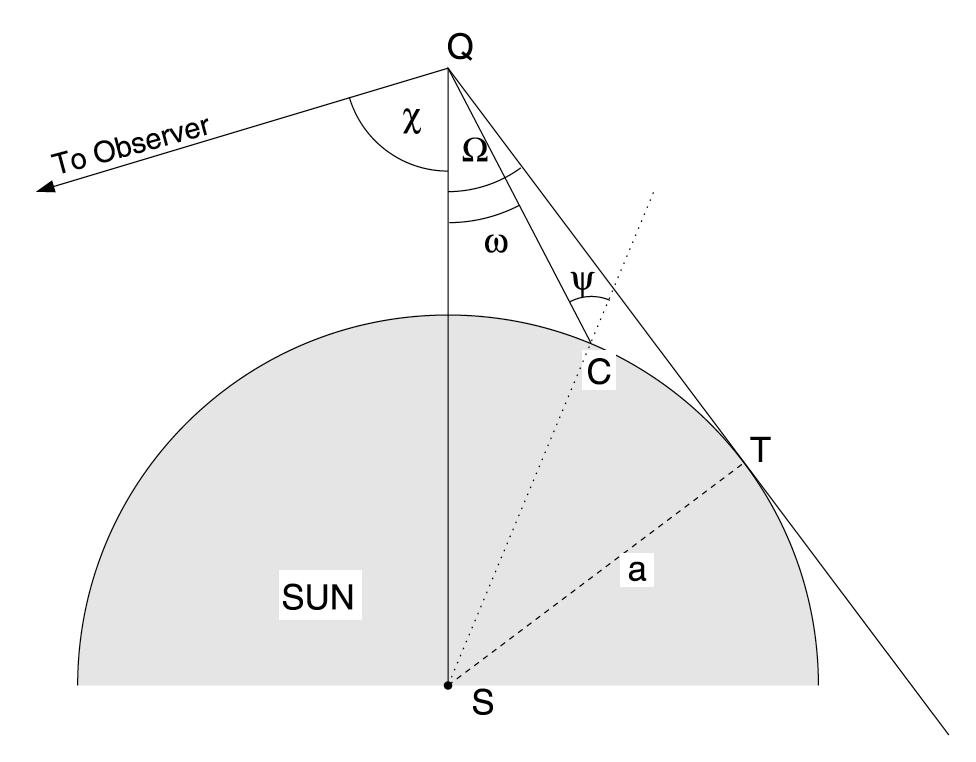
\includegraphics[scale=0.3, angle=0]{images/Omega}
\caption[Coronal Thomson scattering geometry]{Geometry of single electron scattering in the solar atmosphere, with angles $\Omega$ and $\chi$.}
\end{center}
\end{figure}


\subsection{White-light observations of CMEs}\label{sec:11}


\section{Coronagraphs}
Before the early 20th century the only way to view the corona was for a short period during a solar eclipse when the moon blocks direct photospheric light. Under normal conditions direct sunlight overwhelms the faint corona. In 1939 the French Astronomer Bernard Lyot developed a telescope, known as a coronagraph, which allowed observation of the corona at any time \citep{lyot1939}. A coronagraph is an optical system that provides an artificial eclipse of direct photospheric light so the much fainter corona can be imaged.
%A coronagraph is an optical system that provides an artificial eclipse so the faint corona may be imaged at any time. The first working coronagraph was invented by the French astronomer Bernard Lyot in 1930.

\subsection{Lyot Coronagraph}\label{sec:22}
The Lyot Coronagraph is the name given to the first optical design of a coronagraph developed by Bernard Lyot. A basic schematic of the instrument is given in Figure~\ref{fig:lyot}. The optical element O1 is a lens that is extremely polished to prevent scattering and reflections of incident light. O1 creates an image of the Sun onto its focal plane at F1 where the occulting disk, D1, reflects away the unwanted solar disk image. F1 then images the objective lens and the occulting disk onto the plane of O2. Lyot's key invention was the Lyot stop and Lyot spot. These are devices onto which light diffracted at the occulting disk is directed and subsequently blocked from being imaged by the final lens O2. O2 then images the faint corona and occulting disk onto the detector plane. 

The Lyot coronagraph is described as internally occulting due to the placement of the occulting disk behind the first objective lens. This is to distinguish it from a externally occulted system in which the disk is placed in front of the objective lens. Modern coronagraphs follow the same basic design of Lyot's but contain extra features such as baffles to stop any scattered light in the telescope. 

\begin{figure}[!h]
\begin{center}
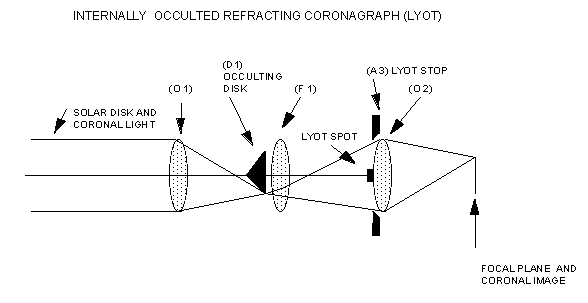
\includegraphics[trim=0cm 1.0cm 0cm 0cm, scale=0.8]{images/Lyot_coronagraph}
\caption[The Lyot coronagraph]{A schematic of the basic optical design of the Lyot coronagraph. Lyot's key inventions where the placement of a Lyot stop and Lyot spot at the positions where diffracted light would contaminate the image and obscure the faint corona.}
\label{fig:lyot}
\end{center}
\end{figure}

\subsection{STEREO COR1 and COR2}\label{sec:22}
The \emph{Solar Terrestrial Relations Observatory} \citep[\emph{STEREO};][]{kai08} Ahead and Behind are two nearly identical spacecraft traveling ahead and behind Earth in its orbit. Each spacecraft is receding from Earth at a rate of $\pm22^{\circ}$ per year, such that they are effectively traveling around the Sun in opposite directions. They carry an identical set of instruments known as the Sun Earth Coronal Connection and Heliospheric Investigation (SECCHI) suite, including in situ detectors and a variety of imagers. On each spacecraft there are two coronagraphs, COR1 and COR2 \citep{how08}. The Ahead COR1 and COR2 combined with Behind COR1 and COR2 offer a stereoscopic view of the corona and any transient event taking place, such as a CME.

COR1 is an internally occulted Lyot coronagraph, see Figure~\ref{fig:COR1_design}. It images the inner corona with a field of view from $1.4 - 4.5\,R_{\odot}$ in a waveband 22.5\,nm wide centered on the H$\alpha$ line at 656\,nm. It has an internal polarizer that takes three images at $0^{\circ}$, $120^{\circ}$, and $240^{\circ}$, so that polarized or total brightness images of the inner corona may be produced. It nominally produces $1024\times1024$ pixel images with platescale of 3.75 arcsec per pixel \citep{thomp2008}. A typical observing sequence will give an image cadence of 10 minutes.

COR2 is an externally occulted Lyot coronagraph. Externally occulted coronagraphs have an extra occulting disk in front of the objective lens, see Figure~\ref{fig:cor2}. This is to prevent direct sunlight scattering off of the objective lens, making internally scattered light less of a problem for this type of coronagraph. A downside to this design is that the external occulter does not allow the inner corona to be imaged, hence such coronagraphs are usually used to observe the extended corona to larger heights. COR2 observes the corona in a field of view from $2.5 - 15\,R_{\odot}$ and in a wavelength range of $650 - 750$\,nm. It nominally produces $2048\times2048$ images, with 14.7 arsec per pixel. Like COR1 it has an internal polarizer producing three linearly polarized images per observing sequence (30 minutes).

These white light imagers of the corona allow for a stereoscopic view of CMEs in a total field of view covering $1.4 - 15\,R_{\odot}$. The two viewpoint capabilities of these telescopes offer a more accurate observational estimation of both CME kinematics and CME mass, resulting in a better understanding of CME dynamics.
\begin{figure}[!t]
\begin{center}
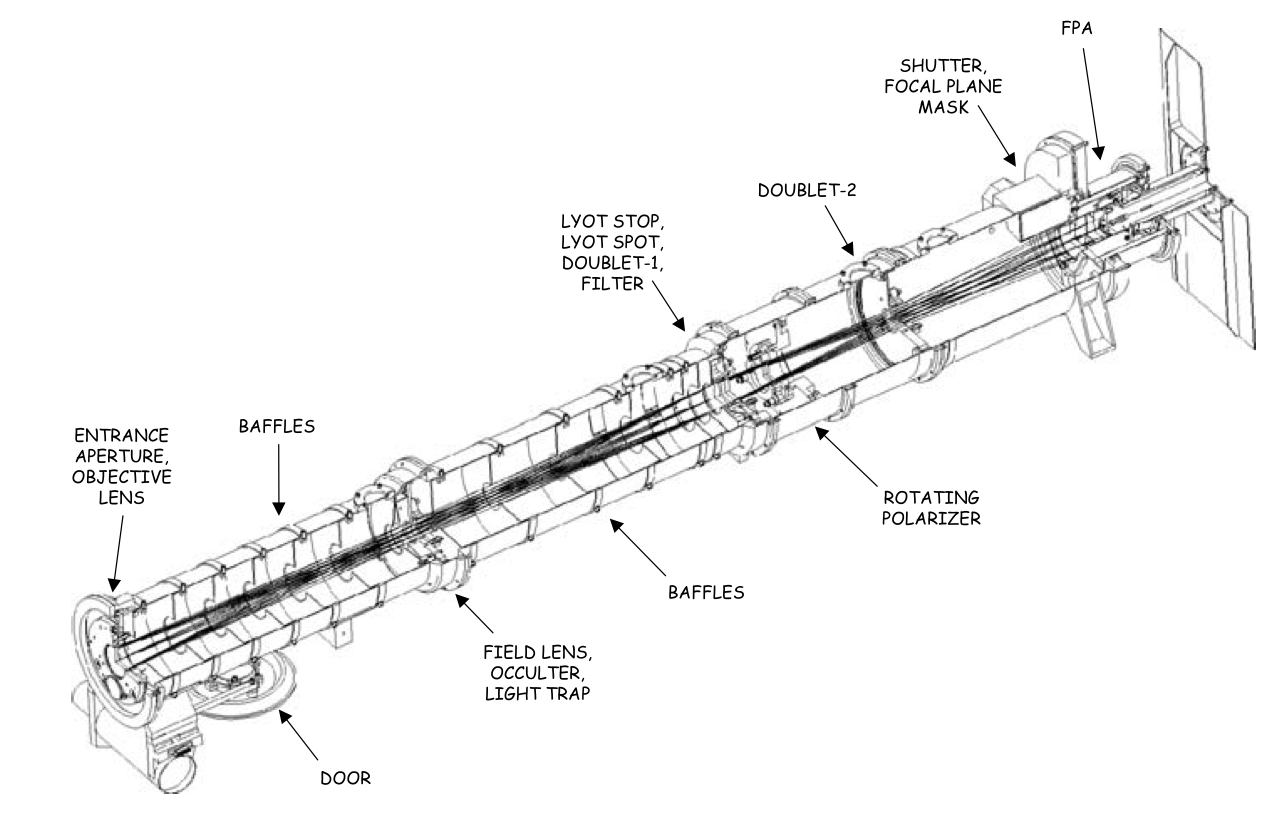
\includegraphics[width=0.95\textwidth]{images/COR1_design}
\caption[The COR1 coronagraph]{A schematic of the basic optical design of the the COR1 coronagraph. There are two such identical instruments, one on the Ahead and one on the Behind spacecraft. It is the same basic design as the Lyot coronagraph with the addition of baffles to prevent scattered light and a polarizer behind the Lyot stop \citep{thomp2008}.}
\label{fig:COR1_design}
\end{center}
\end{figure}
\begin{figure}[!t]
\begin{center}
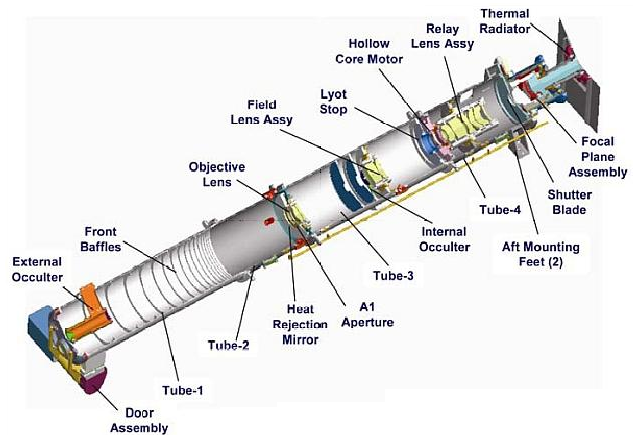
\includegraphics[width=0.9\textwidth]{images/cor2}
\caption[The COR2 coronagraph]{A schematic of the basic optical design of the COR2 coronagraph. This is an externally occulted coronagraph, meaning it has an extra occultation disk in front of the objective lens. This results in less internally scattered light, but also results in an obscuration of the inner corona. As with COR1, there are two such identical instruments, one on the Ahead and one on the Behind spacecraft \citep{how08}.}
\label{fig:cor2}
\end{center}
\end{figure}


\subsection{SOHO LASCO}\label{sec:23}




\section{Radio Spectrometers and Radioheliographs}\label{sec:3}

\subsection{RSTO Callisto}\label{sec:30}

\subsection{STEREO WAVES}\label{sec:31}

\subsection{Nancay Decametric Array}\label{sec:32}

\subsection{Nancay Radioheliograph}\label{sec:33}



\section{EUV imaging}\label{sec:4}

\subsection{SDO AIA}\label{sec:40}



